\section{MPI}\label{sec:mpi}

\subsection{Implementation Strategy}
The Message Passing Interface (MPI) paradigm was used to explore distributed-memory parallelization. Unlike OpenMP, which relies on a shared memory space, MPI requires explicit communication of data between discrete processes. In our approach, the workload was distributed by splitting the first matrix, $A$, by rows among the available processes using \texttt{MPI\_Scatterv}. Since each process needs the full second matrix $B$ to compute its respective rows of the resulting matrix $C$, $B$ was fully broadcasted to all nodes via \texttt{MPI\_Bcast}. Finally, the local results were collected back to the master process using \texttt{MPI\_Gatherv}. 

\begin{lstlisting}[style=CStyle, caption={Optimized kernel i-k-j executed by each MPI process.}, label={lst:mpi_kernel}]
for (int i = 0; i < my_rows; i++) {
    for (int k = 0; k < N; k++) {
        double temp = local_A[i][k];
        for (int j = 0; j < N; j++) {
            local_C[i][j] += temp * B[k][j];
        }
    }
}
\end{lstlisting}

While MPI is natively designed for physical distributed clusters, executing it on a single shared-memory machine highlights the overheads inherently introduced by message passing. By default, MPI implementations do not implicitly share memory among processes on the same host. This drastically increases the RAM footprint (as each process allocates its own full copy of matrix $B$) and introduces substantial data duplication and context-switching penalties that simulate network traffic over the memory bus.

\subsection{Performance and Scalability Analysis}
The algorithm was benchmarked across various matrix sizes ranging from $N = 1024$ up to massive workloads of $N = 15000$, using a number of processes ranging from 1 to 32. 

\begin{figure}[H]
    \centering
    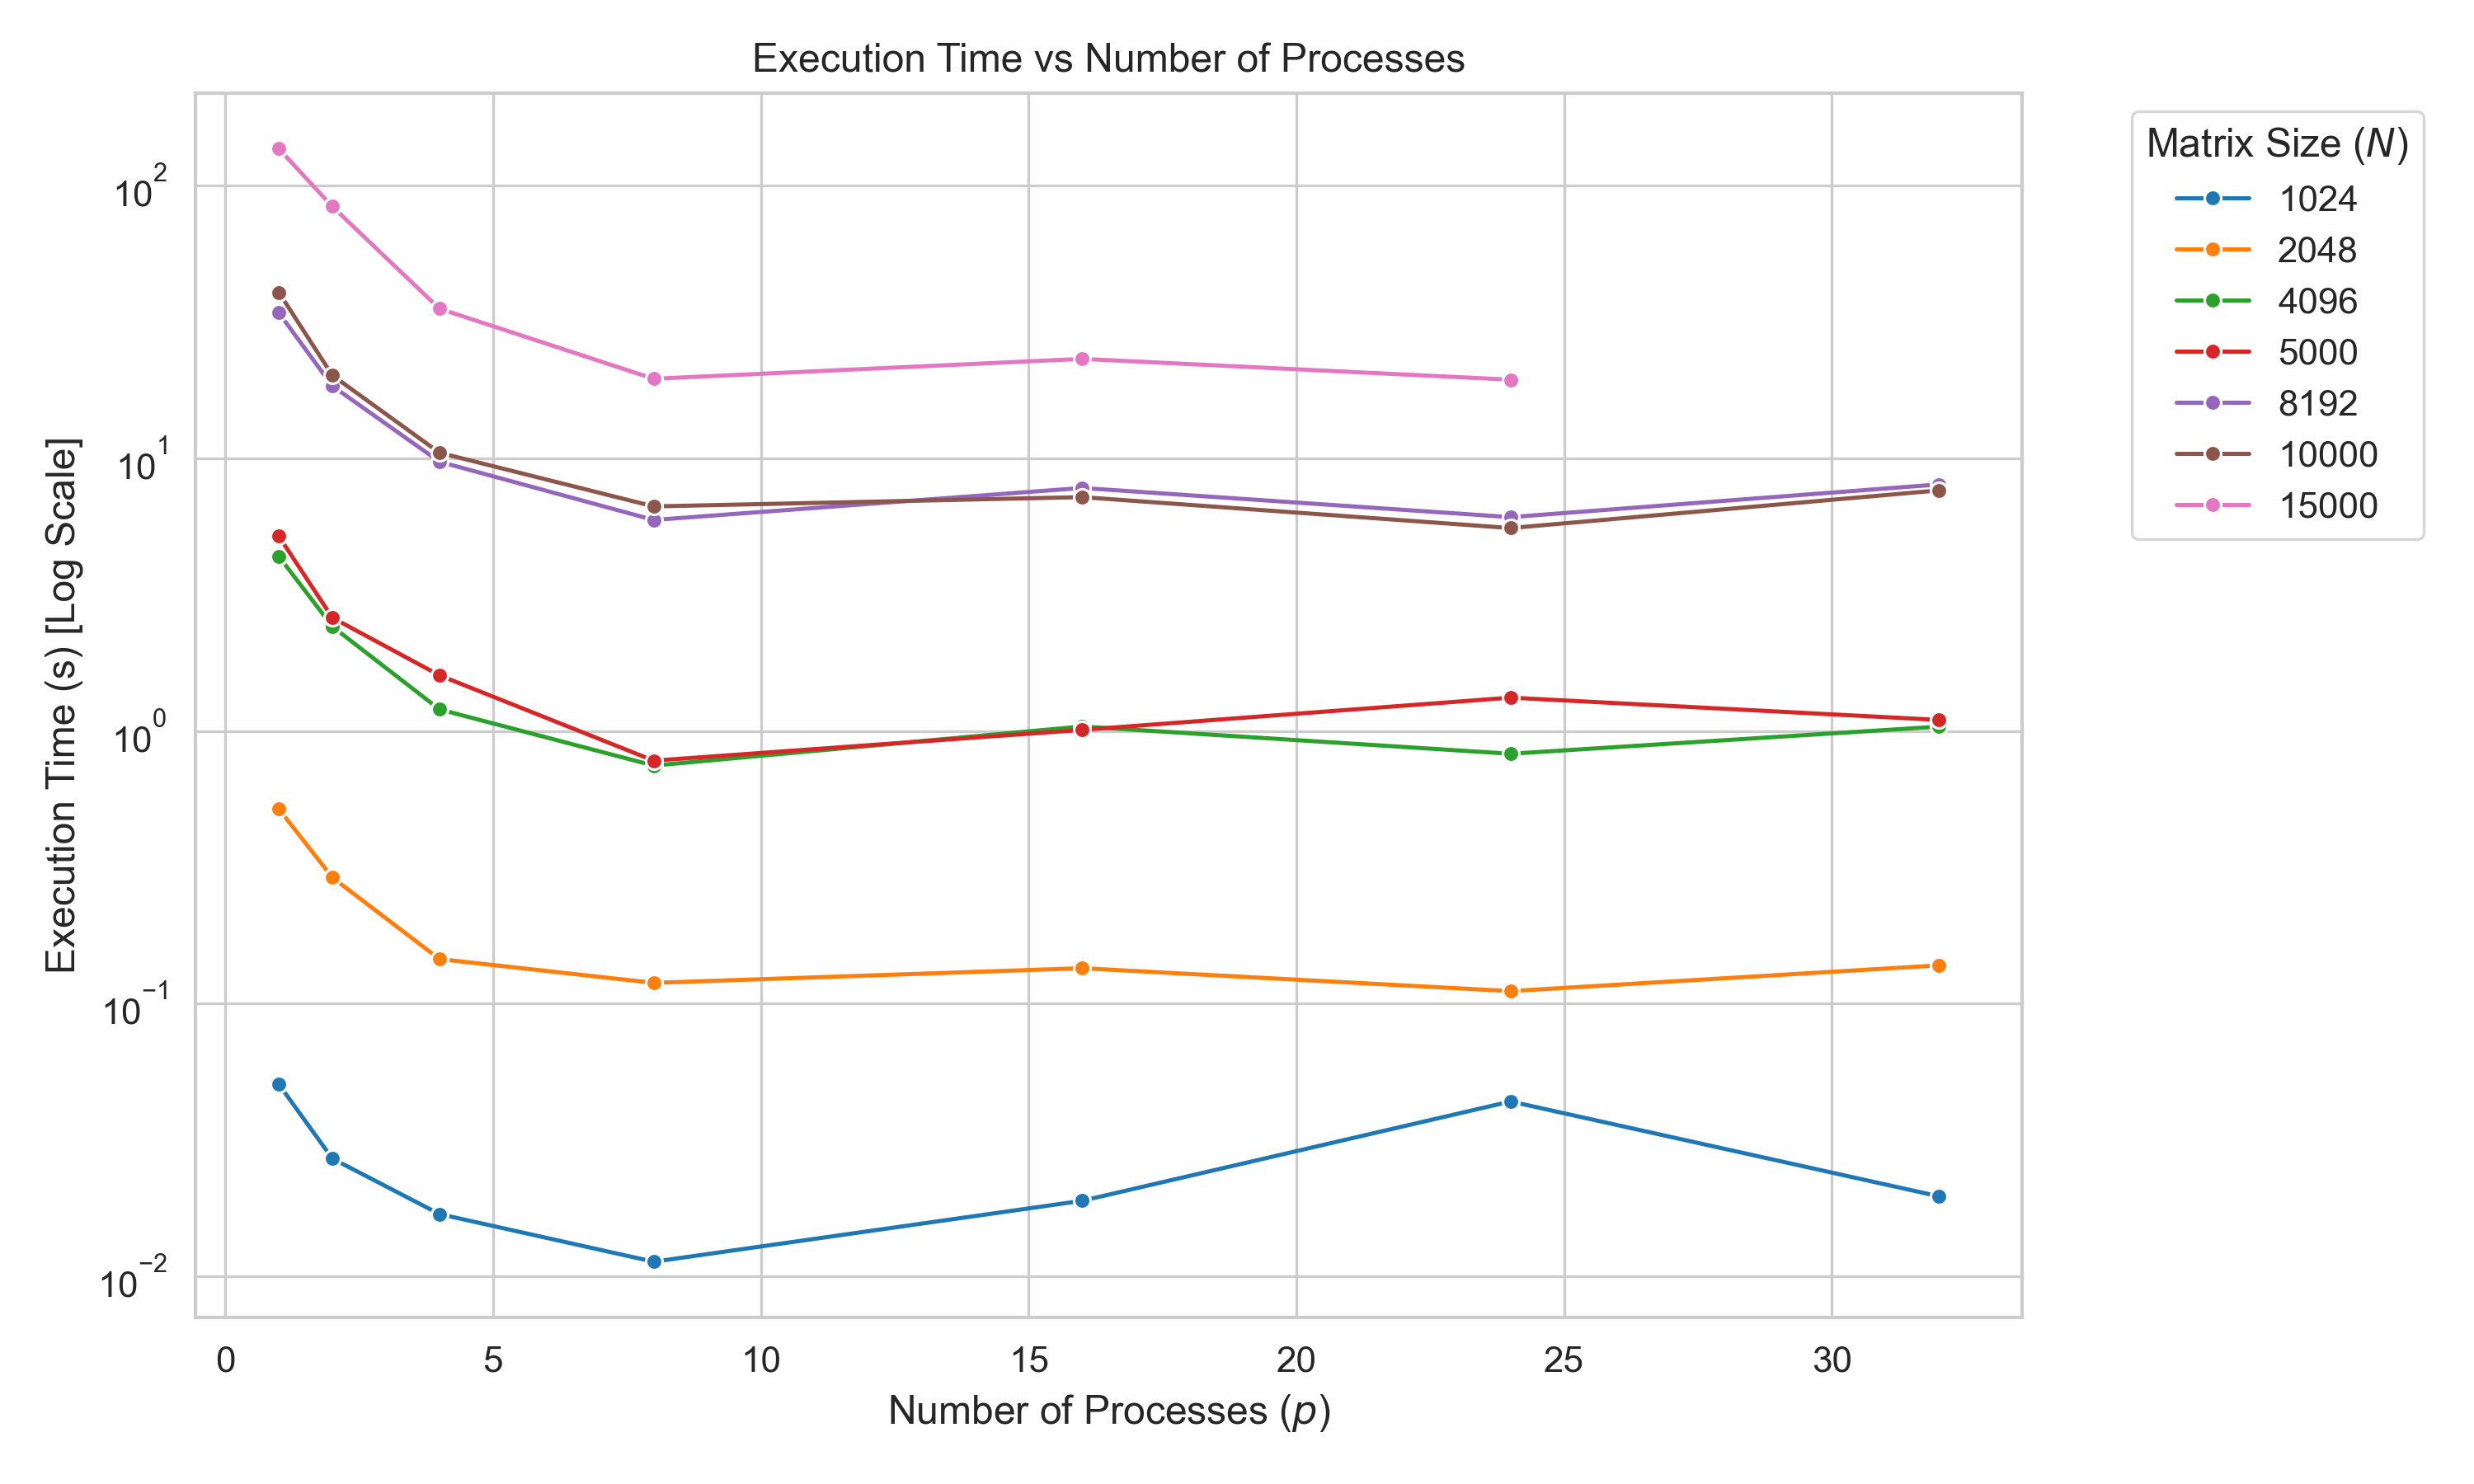
\includegraphics[width=0.8\textwidth]{Images/mpi-plot_1_execution_time.png}
    \caption{Execution time compared to number of processes.}
    \label{fig:mpi_execution_time}
\end{figure} 

The execution time results, shown in Figure~\ref{fig:mpi_execution_time}, demonstrate a consistent performance improvement as the number of processes increases, up to a specific hardware-bound threshold. For $N = 8192$, the sequential baseline execution time was 34.24 seconds, which dropped dramatically to 5.95 seconds at $p=8$. 

Extending the tests to critical dimensions ($N = 10000$ and $N = 15000$) reveals an interesting asymptotic behavior. While for smaller matrices the communication overhead dominates as early as $p=8$, for massive workloads the system benefits from a higher core count, reaching peak performance at $p=24$ for $N=10000$ (5.56s) and $N=15000$ (19.46s).

\begin{figure}[H]
    \centering
    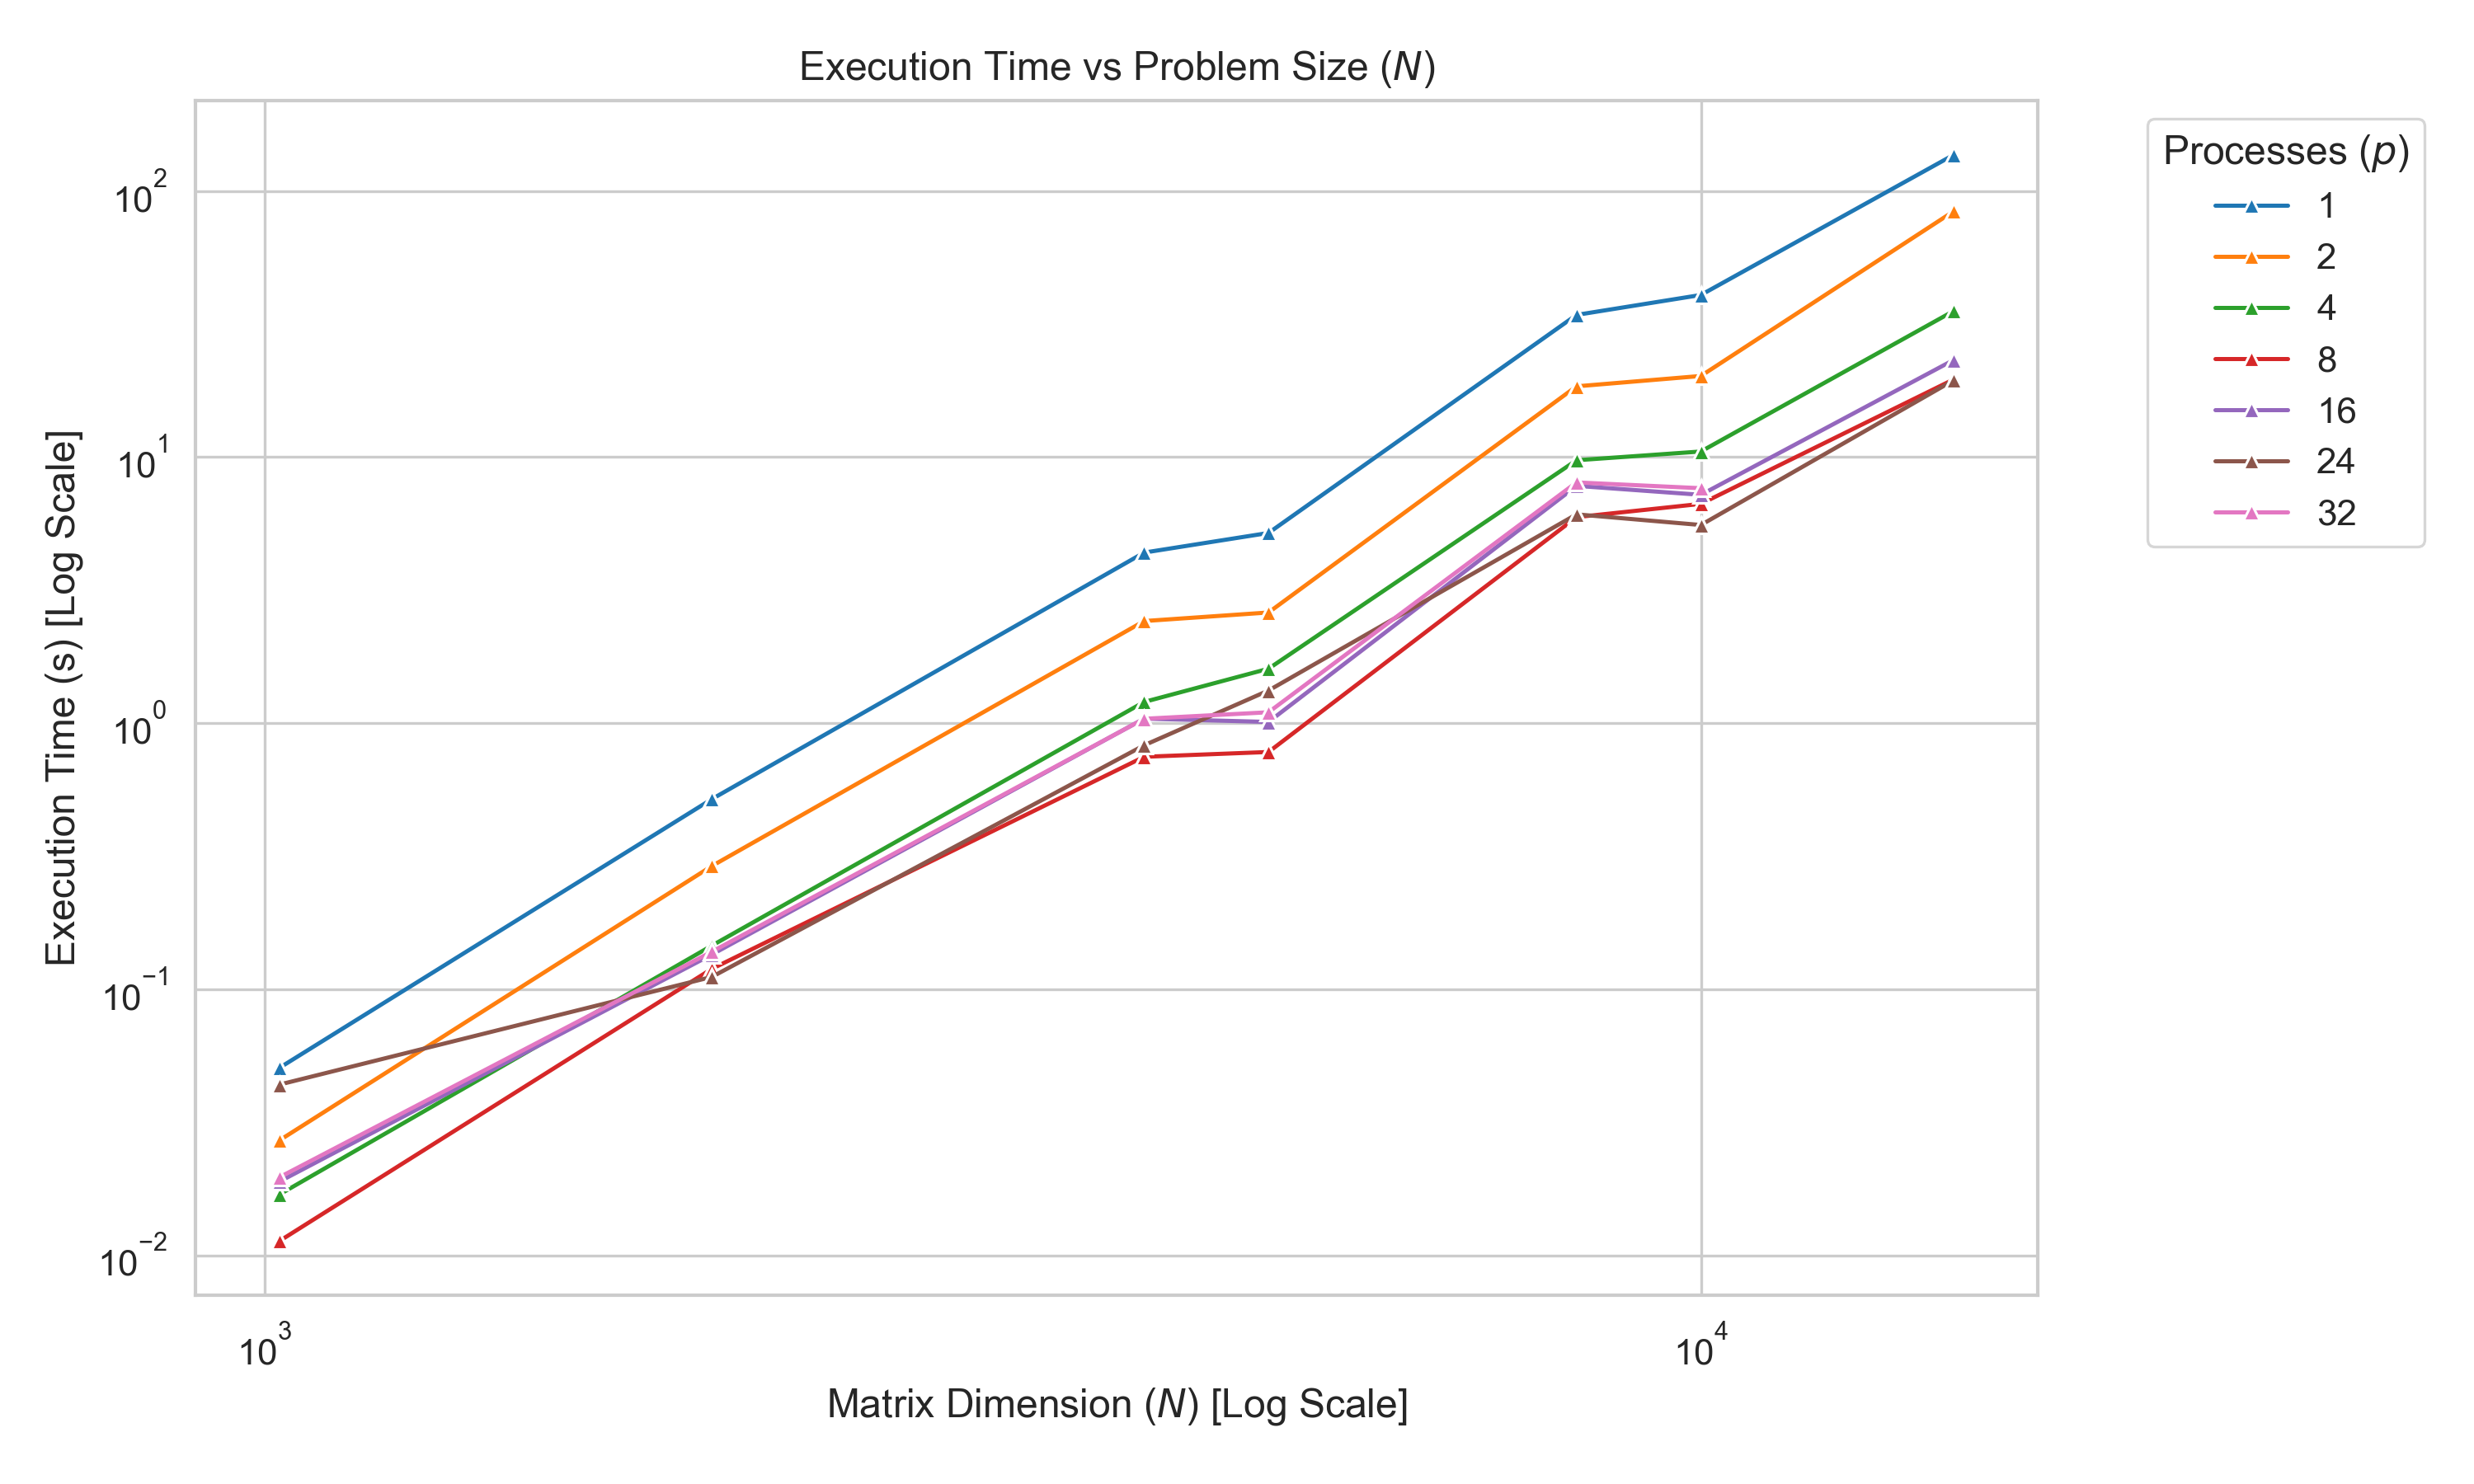
\includegraphics[width=0.8\textwidth]{Images/mpi-plot_5_time_vs_n.png}
    \caption{Execution time compared to problem size $N$ (Log-Log Scale).}
    \label{fig:mpi_time_vs_n}
\end{figure} 

Figure~\ref{fig:mpi_time_vs_n} plots the execution time against the matrix dimension $N$ on a logarithmic scale, perfectly illustrating the theoretical $O(N^3)$ computational complexity of the matrix multiplication algorithm, represented by the consistent positive slope across all process counts.

However, a strict physical limit is reached with $N=15000$ at $p=32$: the independent allocation of matrix $B$ across 32 MPI processes completely saturated the available RAM, causing a runtime Out Of Memory (OOM) error. This highlights the main drawback of MPI on shared-memory architectures compared to OpenMP: severe inefficiency in memory resource utilization.

\subsection{Speedup and Efficiency}

To formally evaluate the implementation, we computed the Speedup ($S_p$) and Efficiency ($E_p$) using the standard formulations $$S_p = T_1 / T_p \qquad and \qquad E_p = S_p / p$$

The speedup plot (Figure~\ref{fig:mpi_speedup}) shows clear sub-linear scaling. For $N = 10000$ at $p=24$, we achieved a maximum speedup of $7.32\times$. For smaller matrices, the communication overhead dominates the computation time almost immediately, leading to a flat speedup curve and a rapidly decreasing efficiency.

\begin{figure}[H]
    \centering
    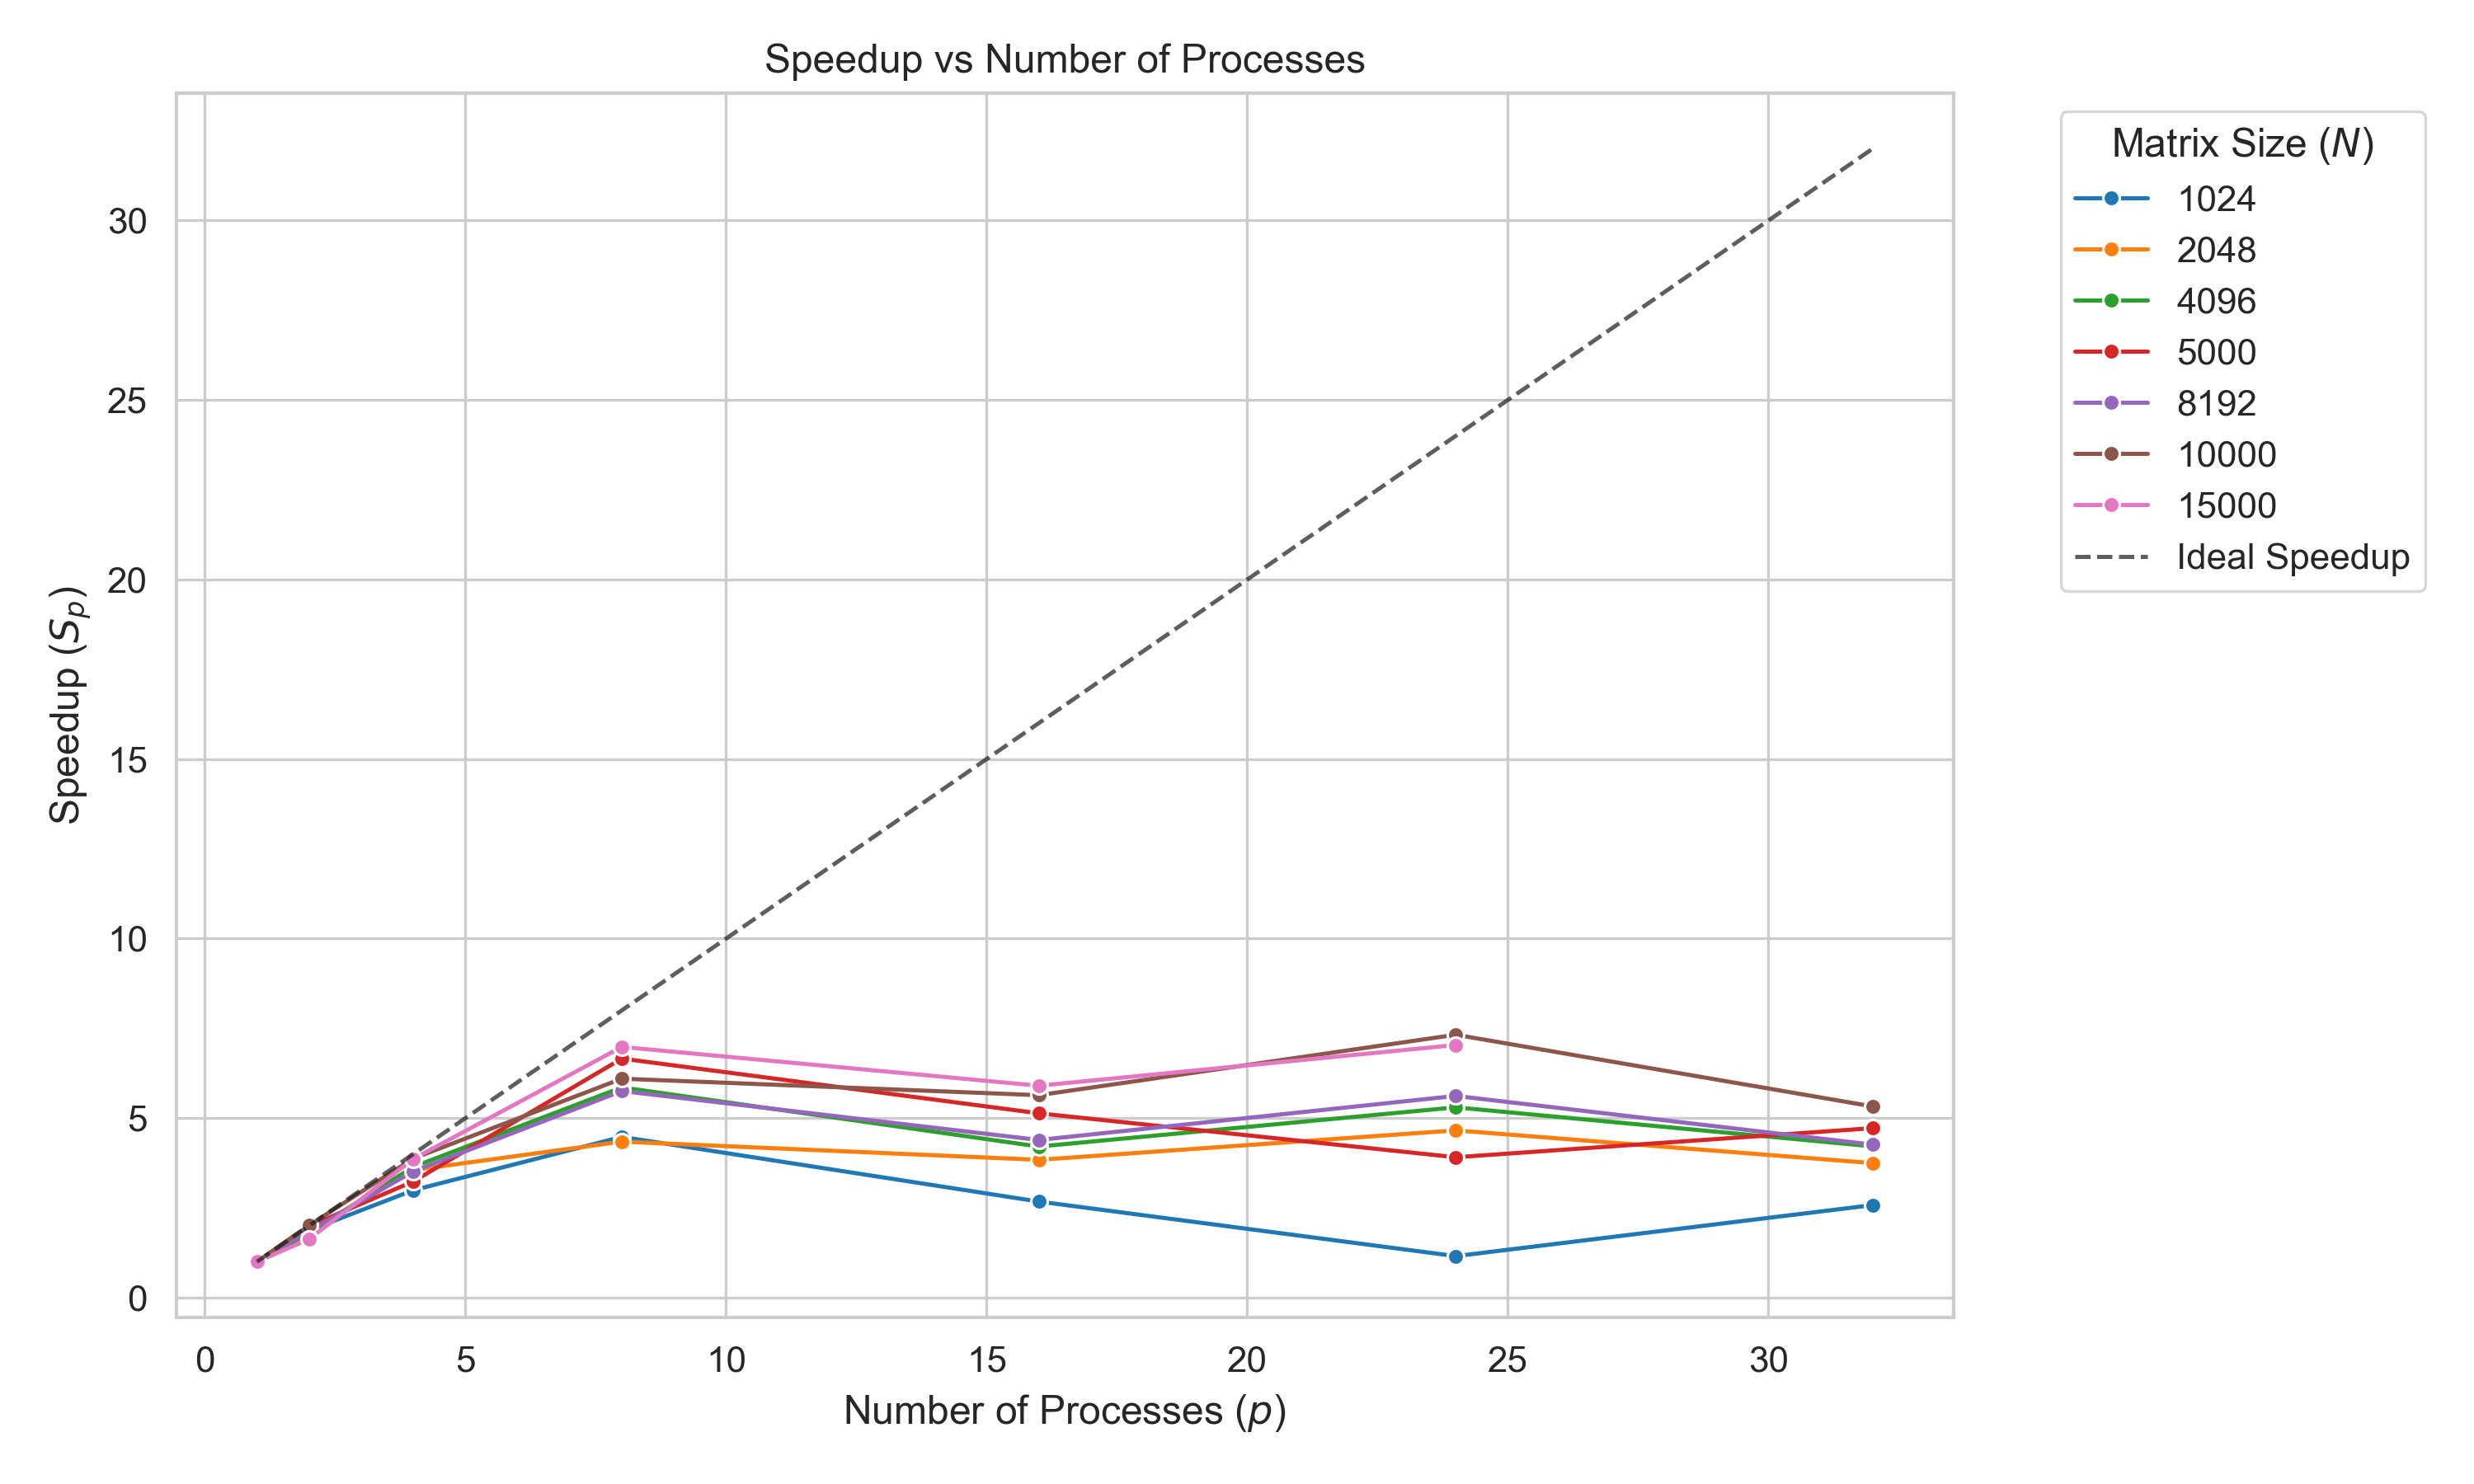
\includegraphics[width=0.8\textwidth]{Images/mpi-plot_2_speedup.png}
    \caption{Speedup compared to number of processes.}
    \label{fig:mpi_speedup}
\end{figure} 

\begin{figure}[H]
    \centering
    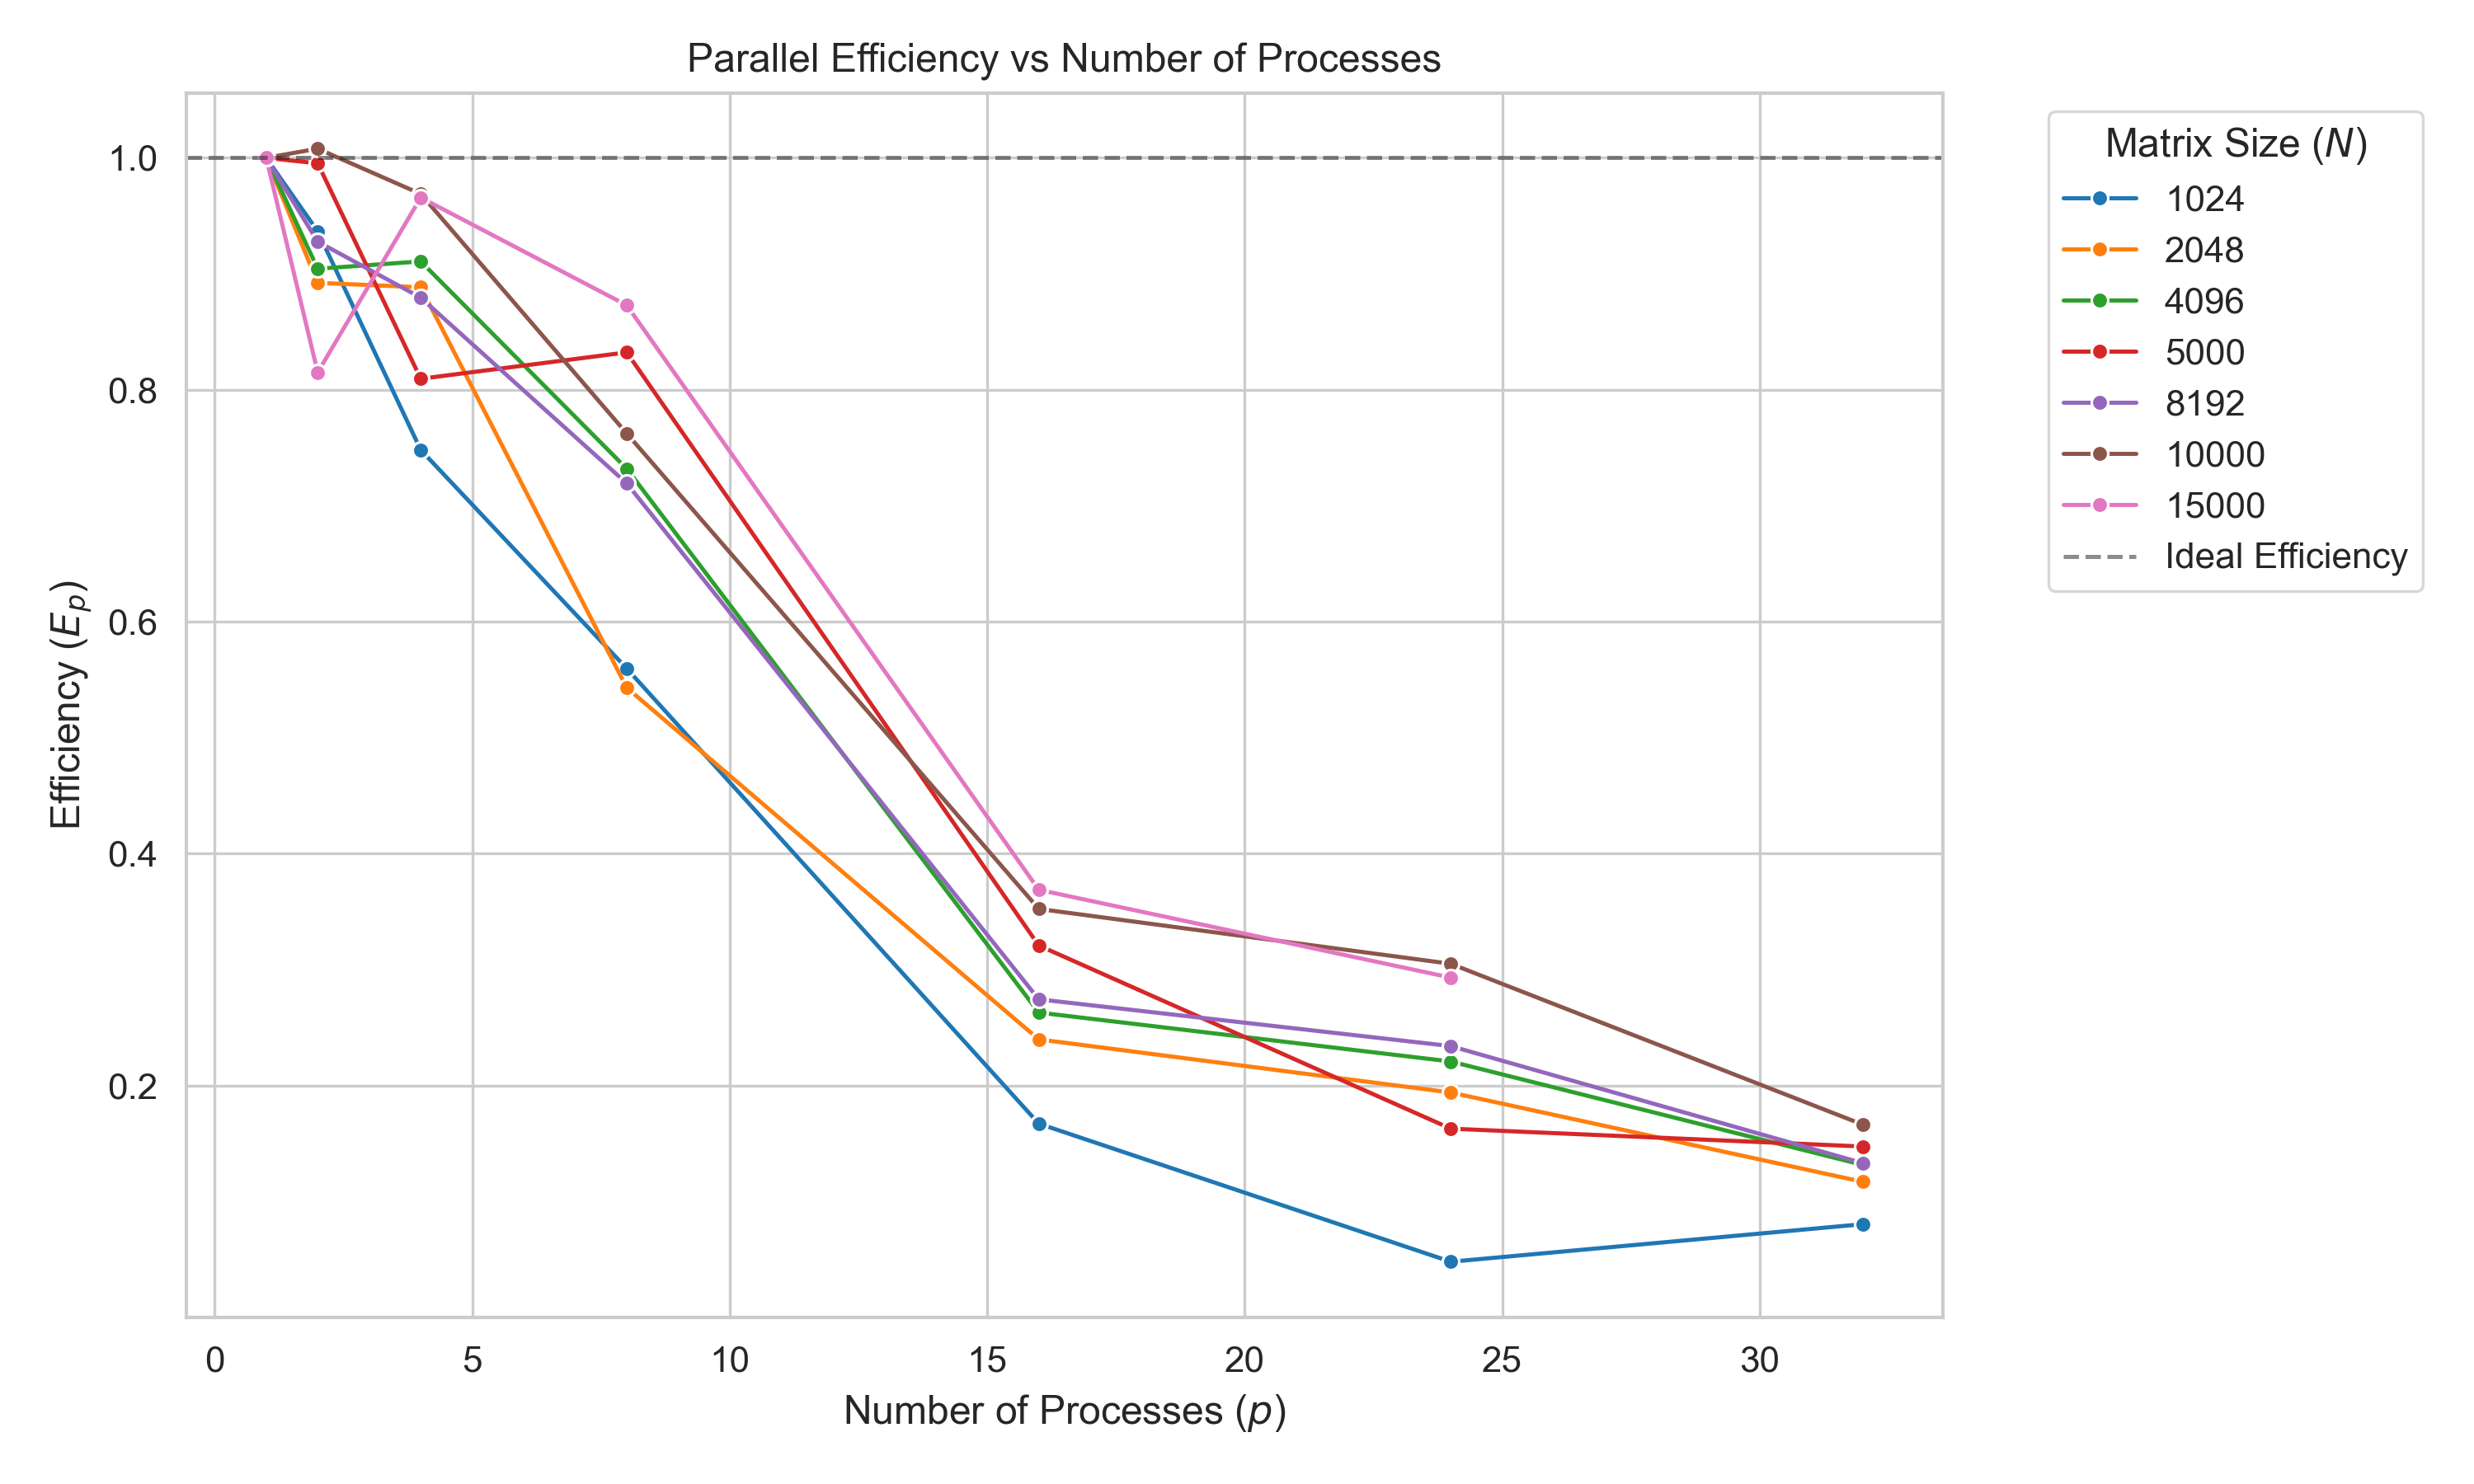
\includegraphics[width=0.8\textwidth]{Images/mpi-plot_3_efficiency.png}
    \caption{Efficiency compared to number of processes.}
    \label{fig:mpi_efficiency}
\end{figure} 

The efficiency heatmap (Figure~\ref{fig:mpi_heatmap}) visualizes the optimal operating window for our MPI implementation. The dark green area indicates that to maintain high efficiency, the problem size can grow but the number of processes must remain "low". When $p$ increases, efficiency drops sharply in the red zone due to inter-process communication dominating execution time.

\begin{figure}[H]
    \centering
    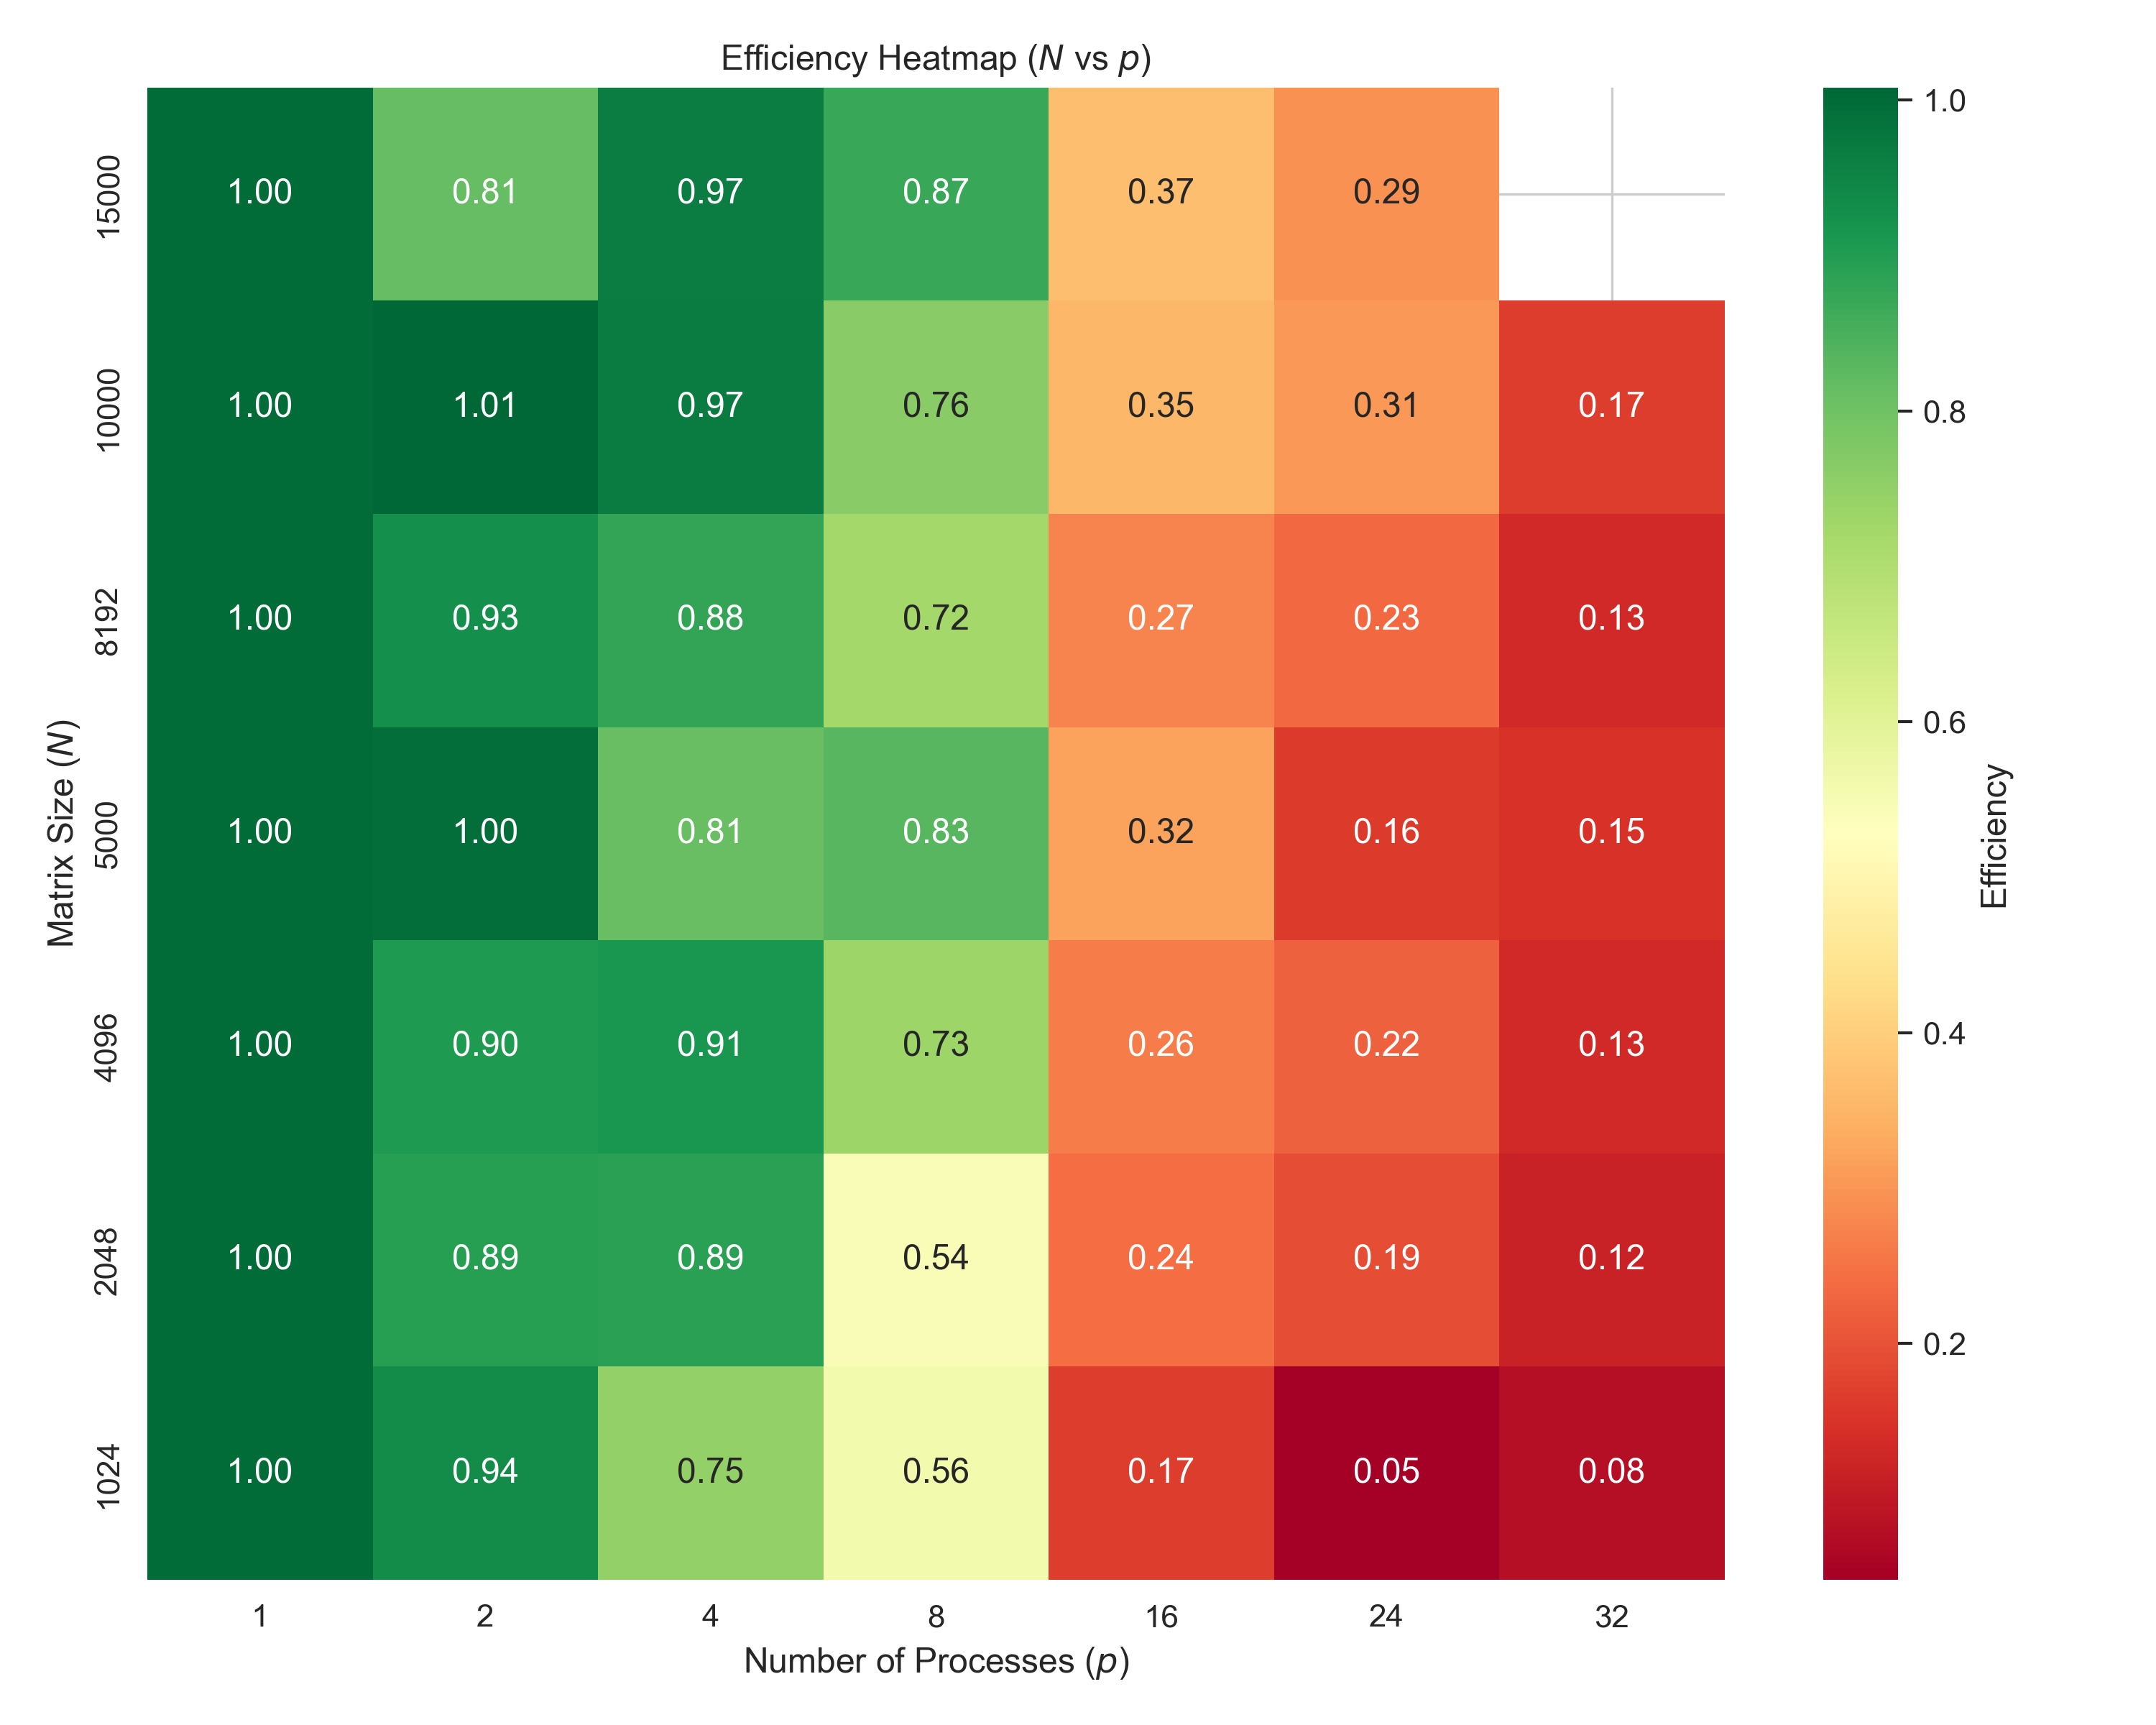
\includegraphics[width=0.75\textwidth]{Images/mpi-plot_6_efficiency_heatmap.png}
    \caption{Efficiency Heatmap mapping the relationship between $N$ and $p$.}
    \label{fig:mpi_heatmap}
\end{figure} 


\subsection{Advanced Throughput and Bottleneck Analysis}

To further assess the hardware utilization and isolate the root causes of the scalability drop, we analyzed the computational throughput and the serial fraction overhead.

\begin{figure}[H]
    \centering
    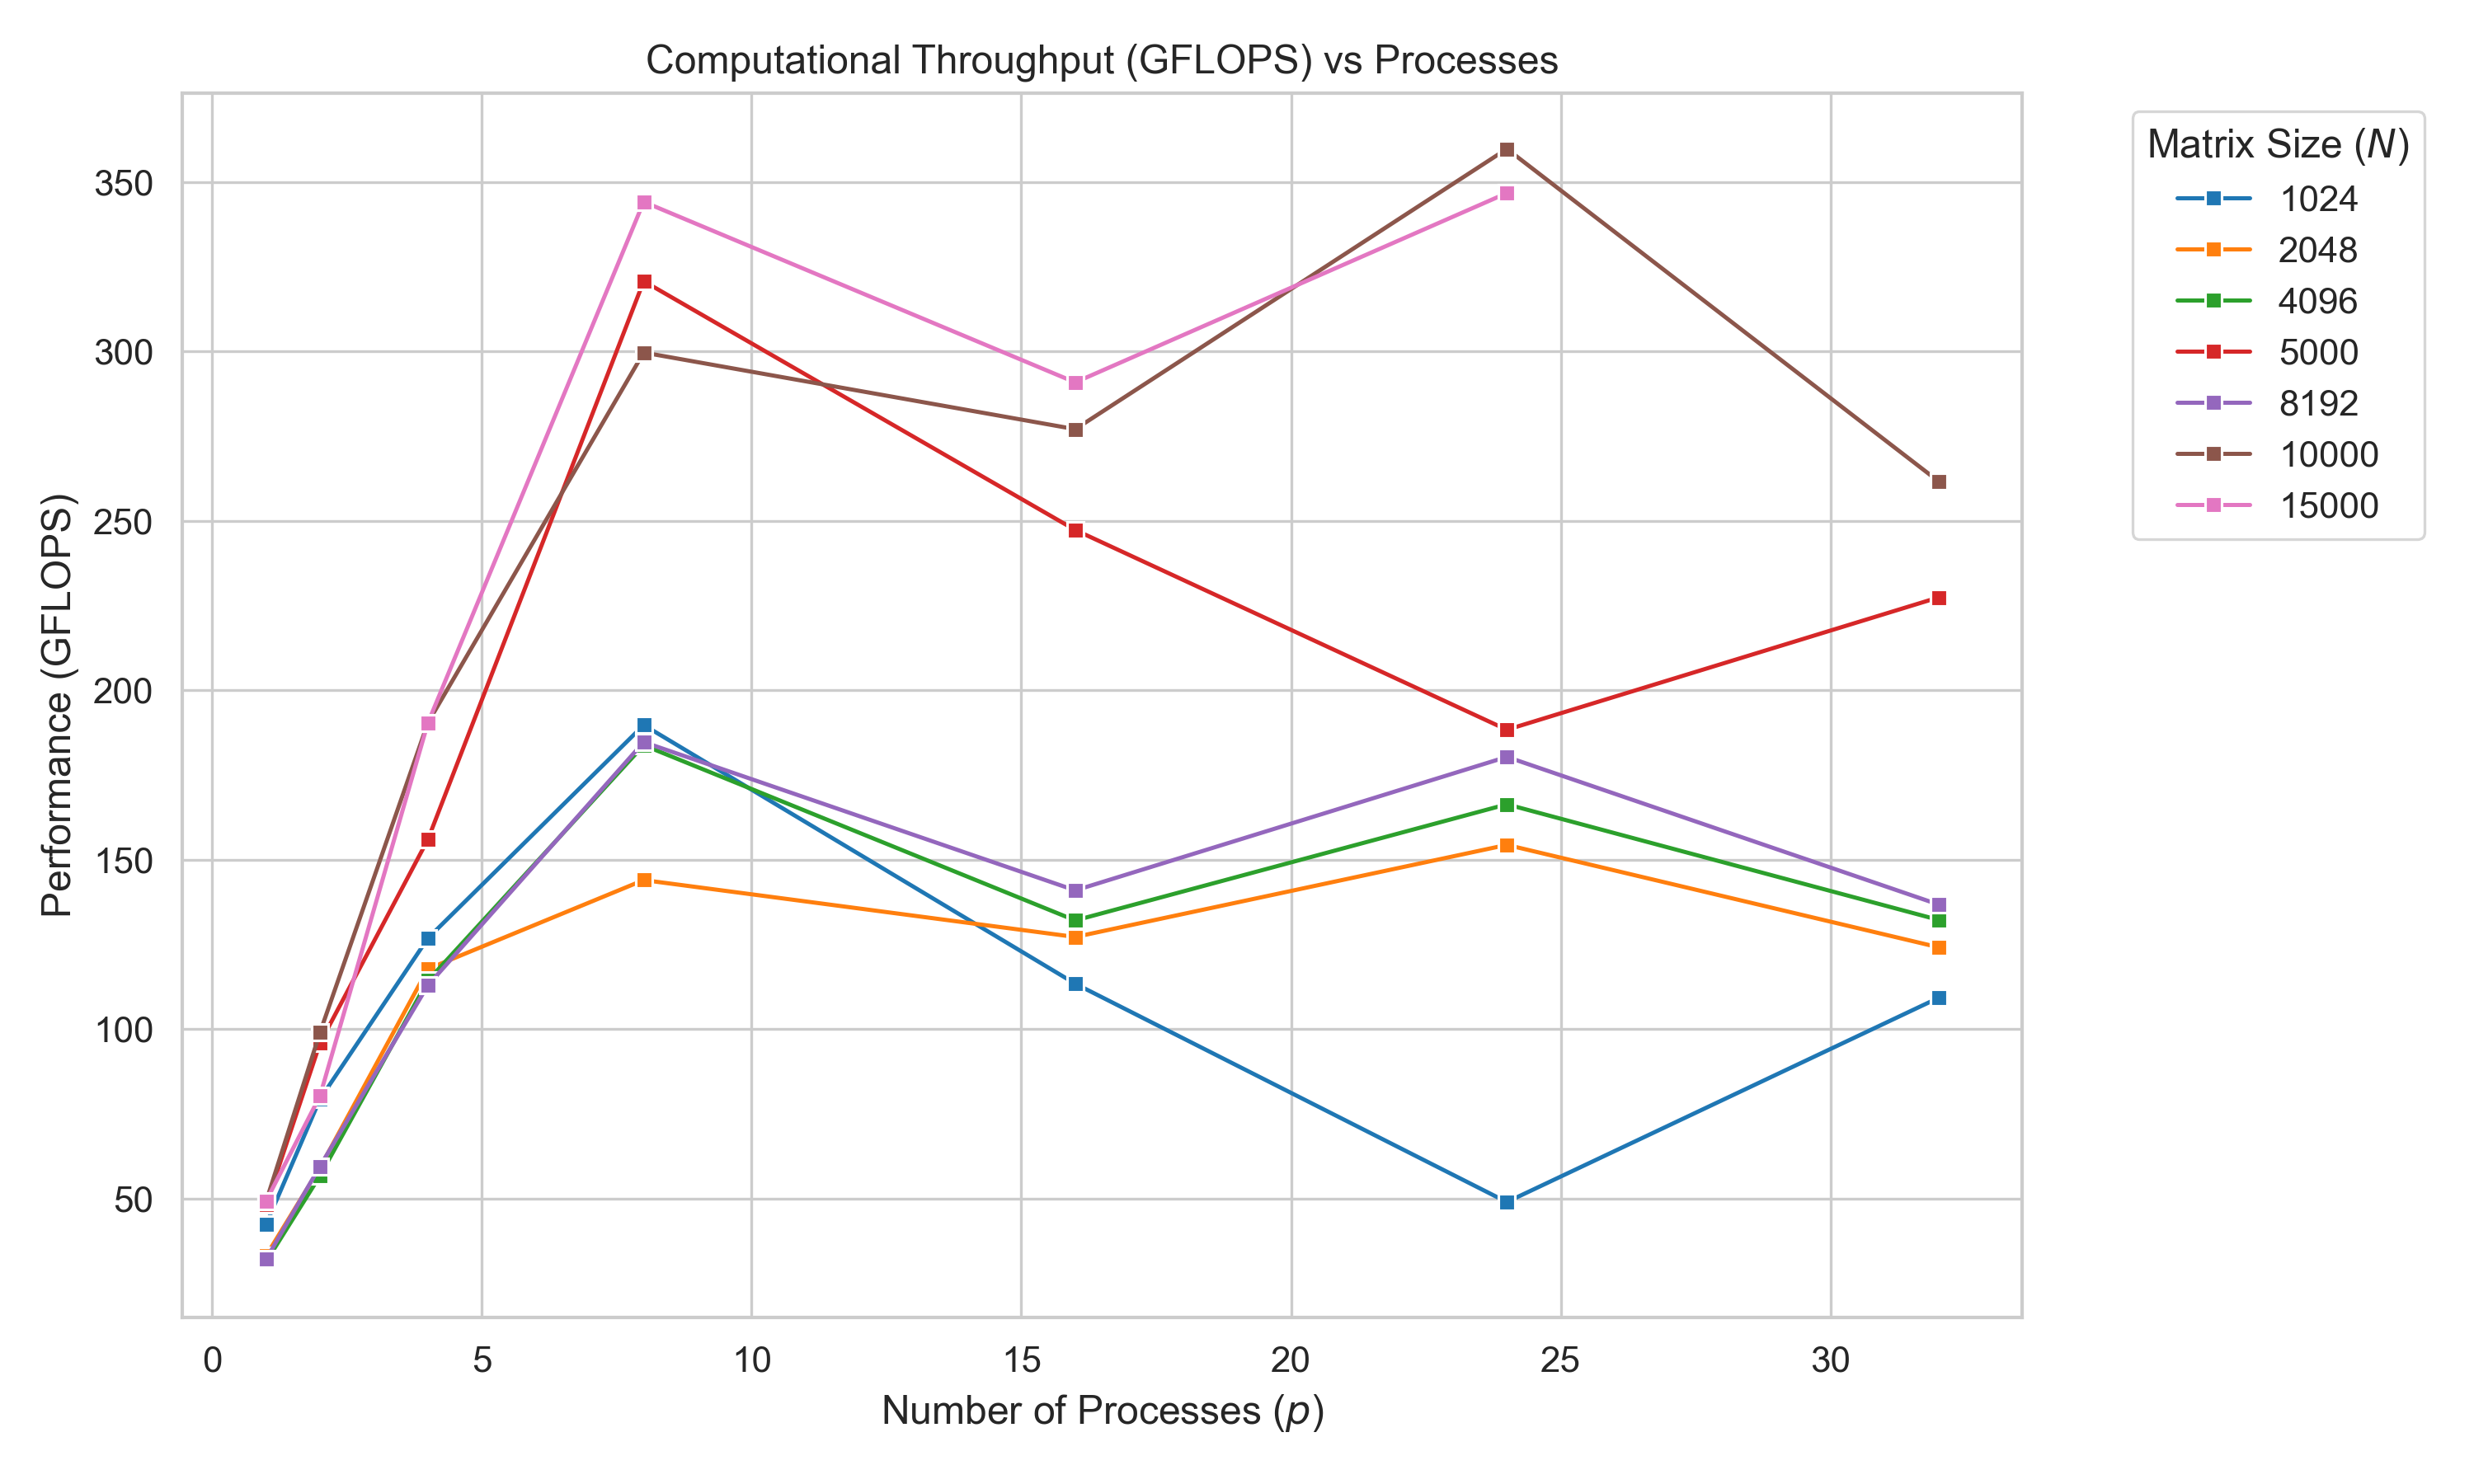
\includegraphics[width=0.8\textwidth]{Images/mpi-plot_4_gflops.png}
    \caption{Computational Throughput (GFLOPS) across different process configurations.}
    \label{fig:mpi_gflops}
\end{figure} 

The GFLOPS chart (Figure~\ref{fig:mpi_gflops}) provides an absolute measure of performance. For small matrices ($N=1024$), the processor barely reaches a few GFLOPS due to constant memory interruption. However, for $N \ge 8192$, the computational throughput scales significantly, demonstrating that the CPU's vector units are being effectively fed with data up until the memory bandwidth saturates.

In conclusion, while the MPI implementation behaves exactly as expected, its deployment on a single machine is definitively bottlenecked by memory bandwidth and data duplication. A physical cluster deployment with high-speed interconnects would be required to mitigate these bounds.

\begin{table}[h!]
\centering
\caption{Complete MPI benchmark results: average execution time (s) across different configurations of processes ($p$) and matrix dimensions ($N$). Note the Out of Memory (OOM) failure for $N=15000$ at $p=32$.}
\label{tab:mpi_final_raw}
\resizebox{\textwidth}{!}{%
\begin{tabular}{@{}lccccccc@{}}
\toprule
\textbf{Configuration} & \textbf{N=1024} & \textbf{N=2048} & \textbf{N=4096} & \textbf{N=5000} & \textbf{N=8192} & \textbf{N=10000} & \textbf{N=15000} \\ \midrule
$p=1$  & 0.0507 & 0.5183 & 4.3779 & 5.1891 & 34.2455 & 40.6978 & 136.9486 \\
$p=2$  & 0.0270 & 0.2904 & 2.4205 & 2.6070 & 18.4566 & 20.1899 & 84.0230 \\
$p=4$  & 0.0169 & 0.1458 & 1.2018 & 1.6025 & 9.7346  & 10.5015 & 35.4518 \\
$p=8$  & 0.0113 & 0.1193 & 0.7476 & 0.7794 & 5.9511  & 6.6733  & 19.6115 \\
$p=16$ & 0.0189 & 0.1350 & 1.0403 & 1.0108 & 7.7987  & 7.2178  & 23.2034 \\
$p=24$ & 0.0438 & 0.1113 & 0.8260 & 1.3271 & 6.0952  & \textbf{5.5584} & \textbf{19.4649} \\
$p=32$ & 0.0197 & 0.1383 & 1.0390 & 1.0992 & 8.0357  & 7.6417  & \text{ERROR} \\ \midrule
\textbf{Optimized (MKL)*} & \textit{\textasciitilde 0.005} & \textit{\textasciitilde 0.04} & \textit{\textasciitilde 0.32} & \textit{\textasciitilde 0.45} & \textit{\textasciitilde 2.5} & \textit{\textasciitilde 4.5} & \textit{\textasciitilde 15.0} \\ \bottomrule
\end{tabular}%
}
\par\smallskip
\small *Theoretical performance estimation using Intel MKL/ScaLAPACK libraries with AVX-512 instructions.
\end{table}